\section{Operads and props}

We consider the category $\Ch$ of chain complexes of abelian groups as our base category, remarking that all definitions in this section apply to general closed symmetric monoidal categories.

\subsection{$\S$-modules and $\S$-bimodules}
Recall that a group $G$ can be thought of as a category with a single object and only invertible morphisms. From this viewpoint, a left $G$-module (resp. right $G$-module or $G$-bimodule) is the same as a functor from $G$ (resp. $G^\op$ or $G \times G^\op$) to $\Ch$.

Let $\S$ be the category whose objects are the natural numbers and whose set of morphisms between $m$ and $n$ is empty if $m \neq n$ and otherwise is the symmetric group $\S_n$.
A \textit{left $\S$-module} (resp. right $\S$-module or $\S$-bimodule) is a covariant functor from $\S$ (resp. $\S^\op$ or $\S \times \S^\op$) to $\Ch$. In this paper we prioritize left module structures over their right counterparts. As usual, taking inverses makes both perspectives equivalent.

The homomorphisms $\S_n \to \S_n \times \S_1$ and $\S_n^\op \to \S_1 \times \S_n^\op$ induce natural forgetful functors $\Uleft$ and $\Uright$ from the category of $\S$-bimodules to those of left and right $\S$-modules.

Given a chain complex $C$ define:
\begin{align*}
\End^C(r) &= \Hom(C, C^{\otimes r})
& \End_C(r) &= \Hom(C^{\otimes r}, C)
&\End^C_C(r, s) &= \Hom(C^{\otimes r}, C^{\otimes s})
\end{align*}
with their natural structures of left $\S$-module, right $\S$-module, and $\S$-bimodule respectively.
The natural forgetful functors from $\S$-bimodules to left and right $\S$-modules send $\End^C_C$ to $\End^C$ and $\End_C$ respectively.

\subsection{Composition structures}

Operads an props are $\S$-modules and \mbox{$\S$-bimodules} respectively enriched with certain composition structures. These are best understood by abstracting the composition structure naturally present in the $\S$-module $\End^C$, naturally an operad, and the $\S$-bimodule $\End^C_C$, naturally a prop.

Succinctly, an operad $\mathcal O$ is an $\S$-module together with a collection of $R$-linear maps
\begin{equation*}
\mathcal O(r) \otimes \mathcal O(s) \to \mathcal O(r+s-1)
\end{equation*}
satisfying suitable associativity, equivariance and unitality conditions.
A prop $\mathcal P$ is an $\S$-bimodule together with two types of compositions; horizontal
\begin{equation*}
\mathcal P(r_1, s_1) \otimes \mathcal P(r_2, s_2) \to \mathcal P(r_1 + r_2, s_1 + s_2)
\end{equation*}
and vertical
\begin{equation*}
\mathcal P(r,s) \otimes \mathcal P(s, t) \to \mathcal P(r, t)
\end{equation*}
satisfying their own versions of associativity, equivariance and unitality.
For a complete presentation of these concepts we refer to Definition 11 and 54 of \cite{Markl08}.

We remark that the compositional structure of a prop $\mathcal P$ restricts to operad structures on $\Uleft(\mathcal P)$ and $\Uright(\mathcal P)$.

%The type of operads that we are most interested in are $E_\infty$-operads which, as we will discuss in the next section, are used to describe commutativity up to coherent homotopies.
%
%\begin{definition} [\cite{may72geometry}, \cite{boardman1973homotopy}]
%	An operad is said to be $E_\infty$ if its underlying \mbox{$\S$-module} is $E_\infty$, and a prop $\mathcal P$ is said to be $E_\infty$ if either $U_1(\mathcal P)$ or $U(\mathcal P)$ is an \mbox{$E_\infty$-operad}.
%\end{definition}

\subsection{Representations}

A morphisms of operads or of props is simply a morphisms of their underlying $\S$-modules or $\S$-bimodules preserving the respective compositional structures.

Consider a chain complex $C$, an operad $\mathcal O$ and a prop $\mathcal P$. An $\mathcal O$-\textit{coalgebra} (resp. $\mathcal O$-\textit{algebra}) structure on $C$ is an operad morphism $\mathcal O \to \End^C$ (resp. $\mathcal O \to \End_C$), and a $\mathcal P$-\textit{bialgebra} structure on $C$ is a prop morphism $\mathcal P \to \End_C^C$.

We remark that the linear duality functor naturally transforms an $\mathcal O$-coalgebra structure on a chain complex into an $\mathcal O$-algebra structure on its dual.

%Algebras over $E_\infty$-operads are the central objects of study in this work. To develop intuition for them, let us consider a chain complex $A$ with an algebra structure over $\underline{R}$, thought of as an operad with all compositions corresponding to the identity map $R \to R$. The $\underline{R}$-algebra structure on $A$ is generated by a linear map $\mu \colon A \otimes A \to A$ which is (strictly) commutative and associative, and a linear map $\eta \colon R \to A$ that determines a (two-sided) unit for $\mu$. Since $E_\infty$-operads are resolutions of $\underline{R}$, their algebras can be thought of as usual unital algebras where the commutativity and associativity relations hold up to coherent homotopies. The two main examples to keep in mind are the cochains of spaces and the chains of infinite loops spaces.	

\subsection{Free operads and props}

We review the definition of the free prop in a symmetric monoidal category $(\mathsf C, \otimes, k)$ generated by an $\S$-bimodule $M$.

An $(m, n)$-graph ... $\mathcal G(m, n)$

Let $I$ and $J$ be finite sets with cardinality $m$ and $n$ respectively.
Define
\begin{equation*}
M(I, J) = \Bij(I, \overline m) \otimes_{\S_m} M(m, n) \otimes_{\S_n} \Bij(I, \overline n).
\end{equation*}
For an $(m, n)$-graph $\Gamma$ we define
\begin{equation*}
F_\Gamma(M)\ =\!\!\! \bigotimes_{v \in Vert(\Gamma)}M(In(v), Out(v)).
\end{equation*}
Notice $F_\Gamma(M)$ is well defined up to isomorphisms induced by the symmetry of the monoidal product.

We can interpret the elements of $M$ as ...

The map $\Gamma \to F_\Gamma(M)$ defines a functor from the groupoid of $(m,n)$-graphs to $\mathsf C$. We define the underlying $\S$-bimodule of the free prop by
\begin{equation*}
F(M)(m, n)\, =\! \colim_{\Gamma \in \mathcal G(m, n)} F_\Gamma(M),
\end{equation*}
where the action ...

The composition structure is given by ...

The unit ...

Universal property ...

The free operad is constructed analogously using ...

\subsection{The prop $\mathcal M$}

Let us consider the symmetric monoidal category of cubical sets $\cSet$. We start by describing three cubical sets respectively modeling: a point, $S^0$, and $S^1$.
\begin{itemize}
	\item[-]$G(1, 0)$ is generated by a cube $\varepsilon$ in dimension $0$.
	\item[-]$G(1, 2)$ has a left action of $\S_2$ and is generated by the cubes $\Delta$ and $(12)\Delta$ in dimension $0$.
	\item[-]$G(2, 1)$ has a right action of $\S_2$ and is generated by a the cubes $\mu$ and $(12)\mu$ in dimension $1$, and $d_0^1 \mu = d_0^1 (12) \mu = d_1^1 \mu$.
\end{itemize}
Let $G$ be the $\S$-bimodule with $G(m, n) = \emptyset$ for biarities not specified above, and let us consider the free prop $F(G)$ generated by it.

Consider the prop morphism $R \colon F(G) \to F(G)$ sending $d_0^0 \mu$ and $d_0^1 \mu$ respectively to
\begin{equation*}
	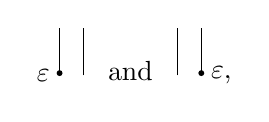
\begin{tikzpicture}[scale=.15]
	\draw (-4,0)--(-4,4);
	\draw (-6,0)--(-6,4);
	\draw [fill] (-6,.2) circle [radius=.2];
	\node [left] at (-6,0) {$\varepsilon$};
	
	\node at (0,.4) {and};
	
	\draw (4,0)--(4,4);
	\draw (6,0)--(6,4);
	\draw [fill] (6,.2) circle [radius=.2];
	\node [right] at (6,0) {$\varepsilon$,};
	\end{tikzpicture}
\end{equation*}
AND THE OTHER TWO RELATIONS. 

We define $\mathcal M$ as the pushout
\begin{equation*}
\begin{tikzcd}
F(G) \arrow[r, "\id"] \arrow[d, "R"'] & F(G) \arrow[d, dashed] \\
F(G) \arrow[r, dashed] & \mathcal M. \\
\end{tikzcd}
\end{equation*}